\documentclass[12pt, fleqn]{article}

\usepackage[left=0.75in, right=0.75in, bottom=0.75in, top=1.0in]{geometry}
\usepackage{amsmath}
\usepackage{amssymb}
\usepackage{amsthm}
\usepackage{mathtools}
\usepackage{hyperref}
\usepackage{ulem}
\usepackage{enumitem}
\usepackage{floatrow}
\usepackage{graphicx}
\usepackage[export]{adjustbox}
\usepackage{sectsty}
% \sectionfont{\centering}
\renewcommand*{\thesubsection}{\alph{subsection}.}

\usepackage[dvipsnames]{xcolor}
\usepackage[perpage]{footmisc}

\usepackage{fancyhdr}
\pagestyle{fancy}
\fancyhf{}
\lhead{190100044}
\rhead{CS 341 Assignment 3}
\renewcommand{\footrulewidth}{1.0pt}
\cfoot{Page \thepage}

\setlength{\parindent}{0em}

\title{CS 341 Assignment 3}
\author{Devansh Jain, 190100044}
\date{\today}

\begin{document}

% \pagenumbering{gobble}
\maketitle
\tableofcontents
\thispagestyle{empty}
\setcounter{page}{0}

\newpage
\section{5 Stage, without forwarding or hazard detection}

\subsubsection*{Code}
\begin{verbatim}
.text

main:
    addi s0 zero 5
    add s1 s0 zero
\end{verbatim}

\subsubsection*{Behaviour}
Expectation: At the end of the program, we expect registers \verb!s0! and \verb!s1! to have value 5. \\
Reality: At the end of the program, only register \verb!s0! has value 5. (\verb!s1! is default to 0)

\subsubsection*{Explanation}
The incorrect value is due to data hazard. \\
To be more specific, we face a \textbf{read-before-write (RAW) data hazard}. \\
\verb!addi s0 zero 5! writes to register \verb!s0! in WB stage during 4th cycle. \\
\verb!add s1 s0 zero! reads from register \verb!s0! in ID stage during 2nd cycle. \\
The value read here is not updated yet causing the incorrect computation.

\subsubsection*{Screenshots}
\begin{figure}[H]
  \centering
  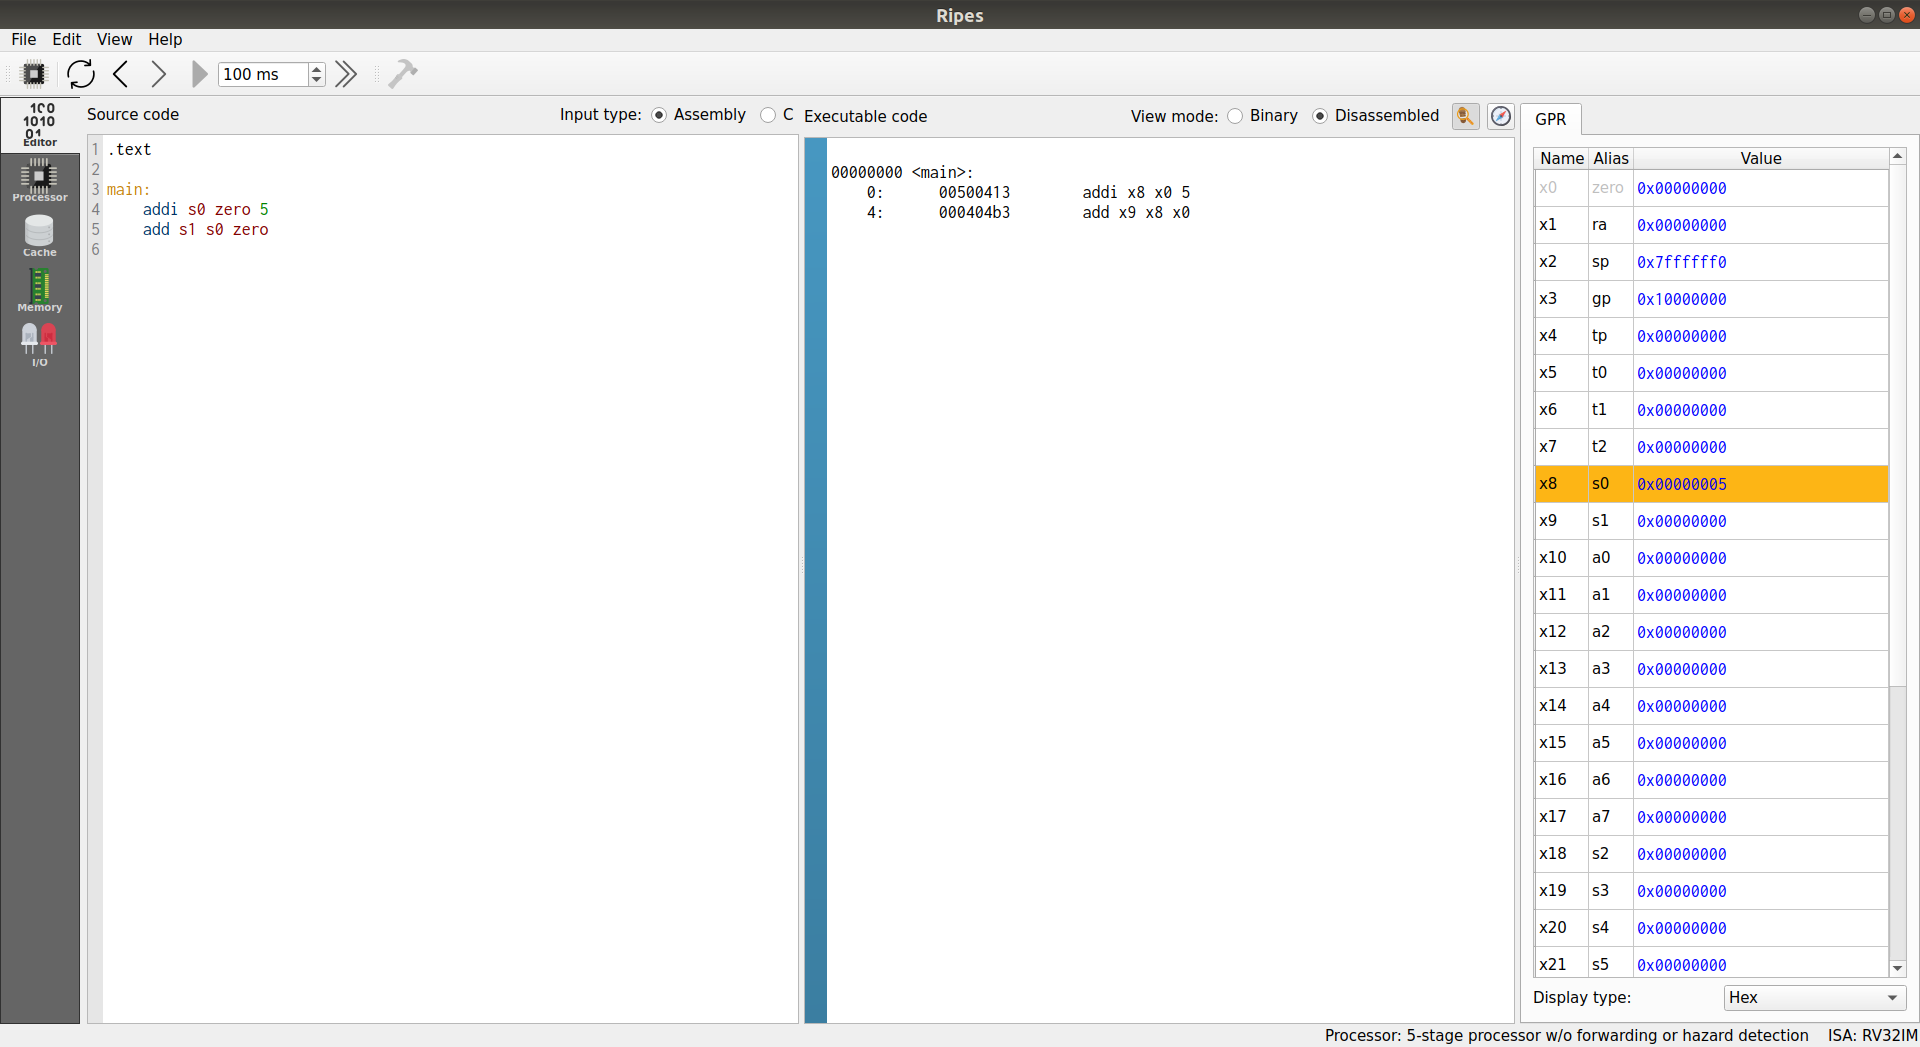
\includegraphics[scale=0.25]{Q1/nhnf_end_editor.png}
  \caption{Without hazard detection; Without forwarding;}
\end{figure}
\begin{figure}[H]
  \centering
  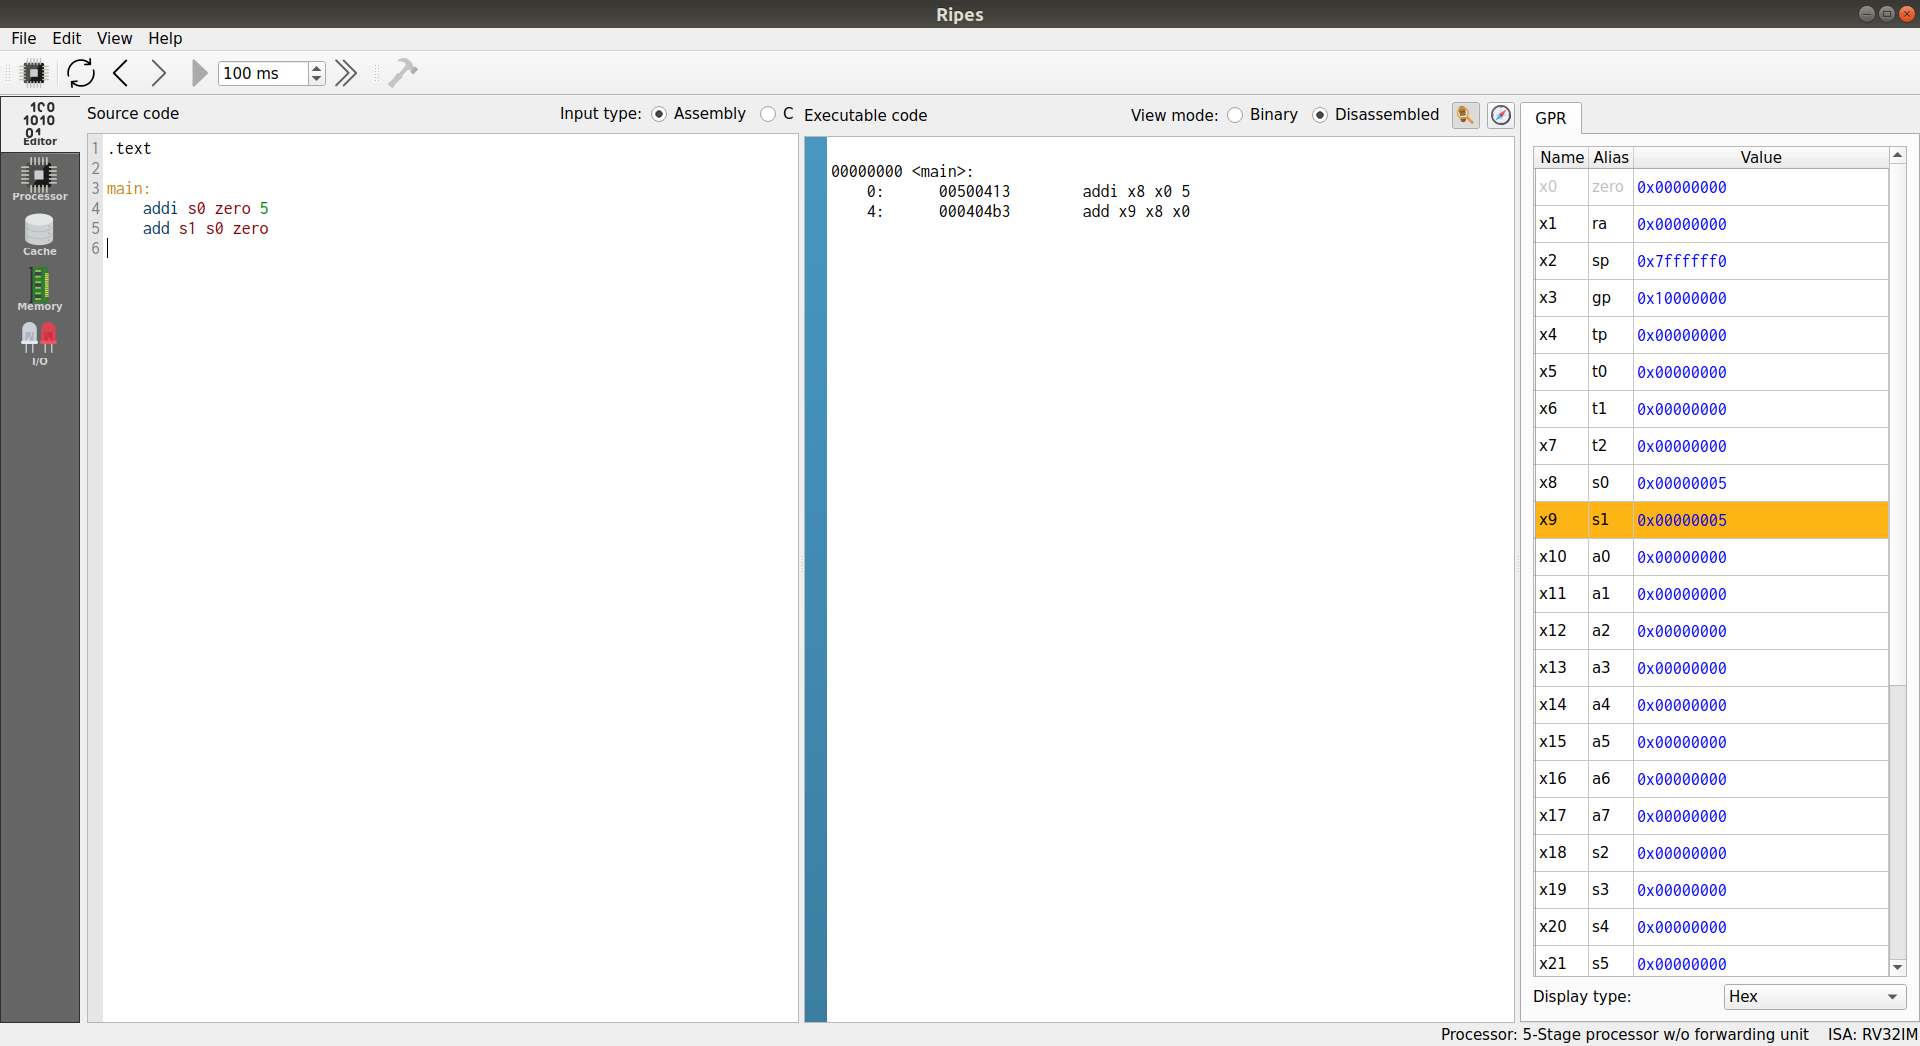
\includegraphics[scale=0.25]{Q1/hnf_end_editor.png}
  \caption{With hazard detection; Without forwarding;}
\end{figure}


\newpage
\section{5 Stage, without forwarding, with hazard detection}

\subsection{}
\subsubsection*{Code}
\begin{verbatim}
.text

main:
    addi s0 zero 5
    add s1 s0 zero
\end{verbatim}

\subsubsection*{Behaviour}
At the end of the program, we expect registers \verb!s0! and \verb!s1! to have value 5. \\
Without forwarding, we observe that ID for second instruction takes 3 cycles (2 stalls). \\
There are no stalls with forwarding.

\subsubsection*{Screenshots}
\begin{figure}[H]
  \centering
  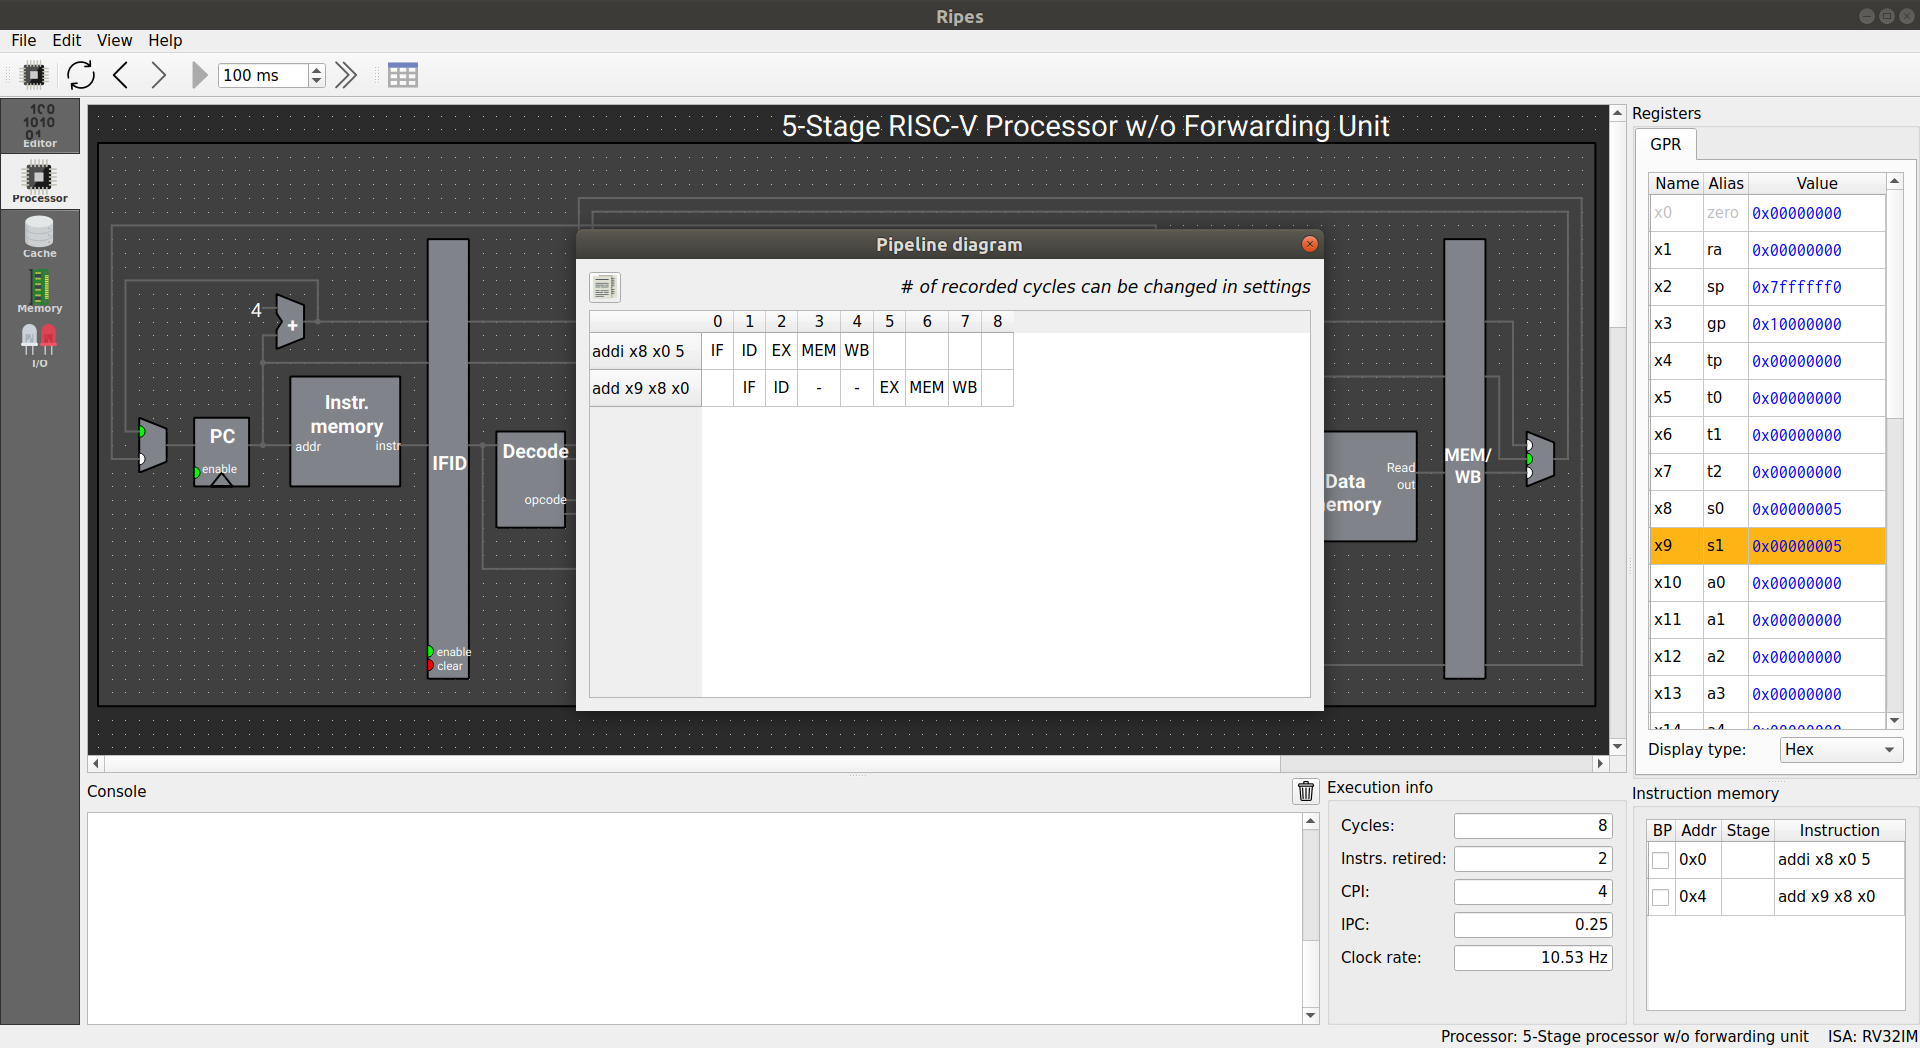
\includegraphics[scale=0.25]{Q2/a_hnf_end_pipeline.png}
  \caption{With hazard detection; Without forwarding;}
\end{figure}
\begin{figure}[H]
  \centering
  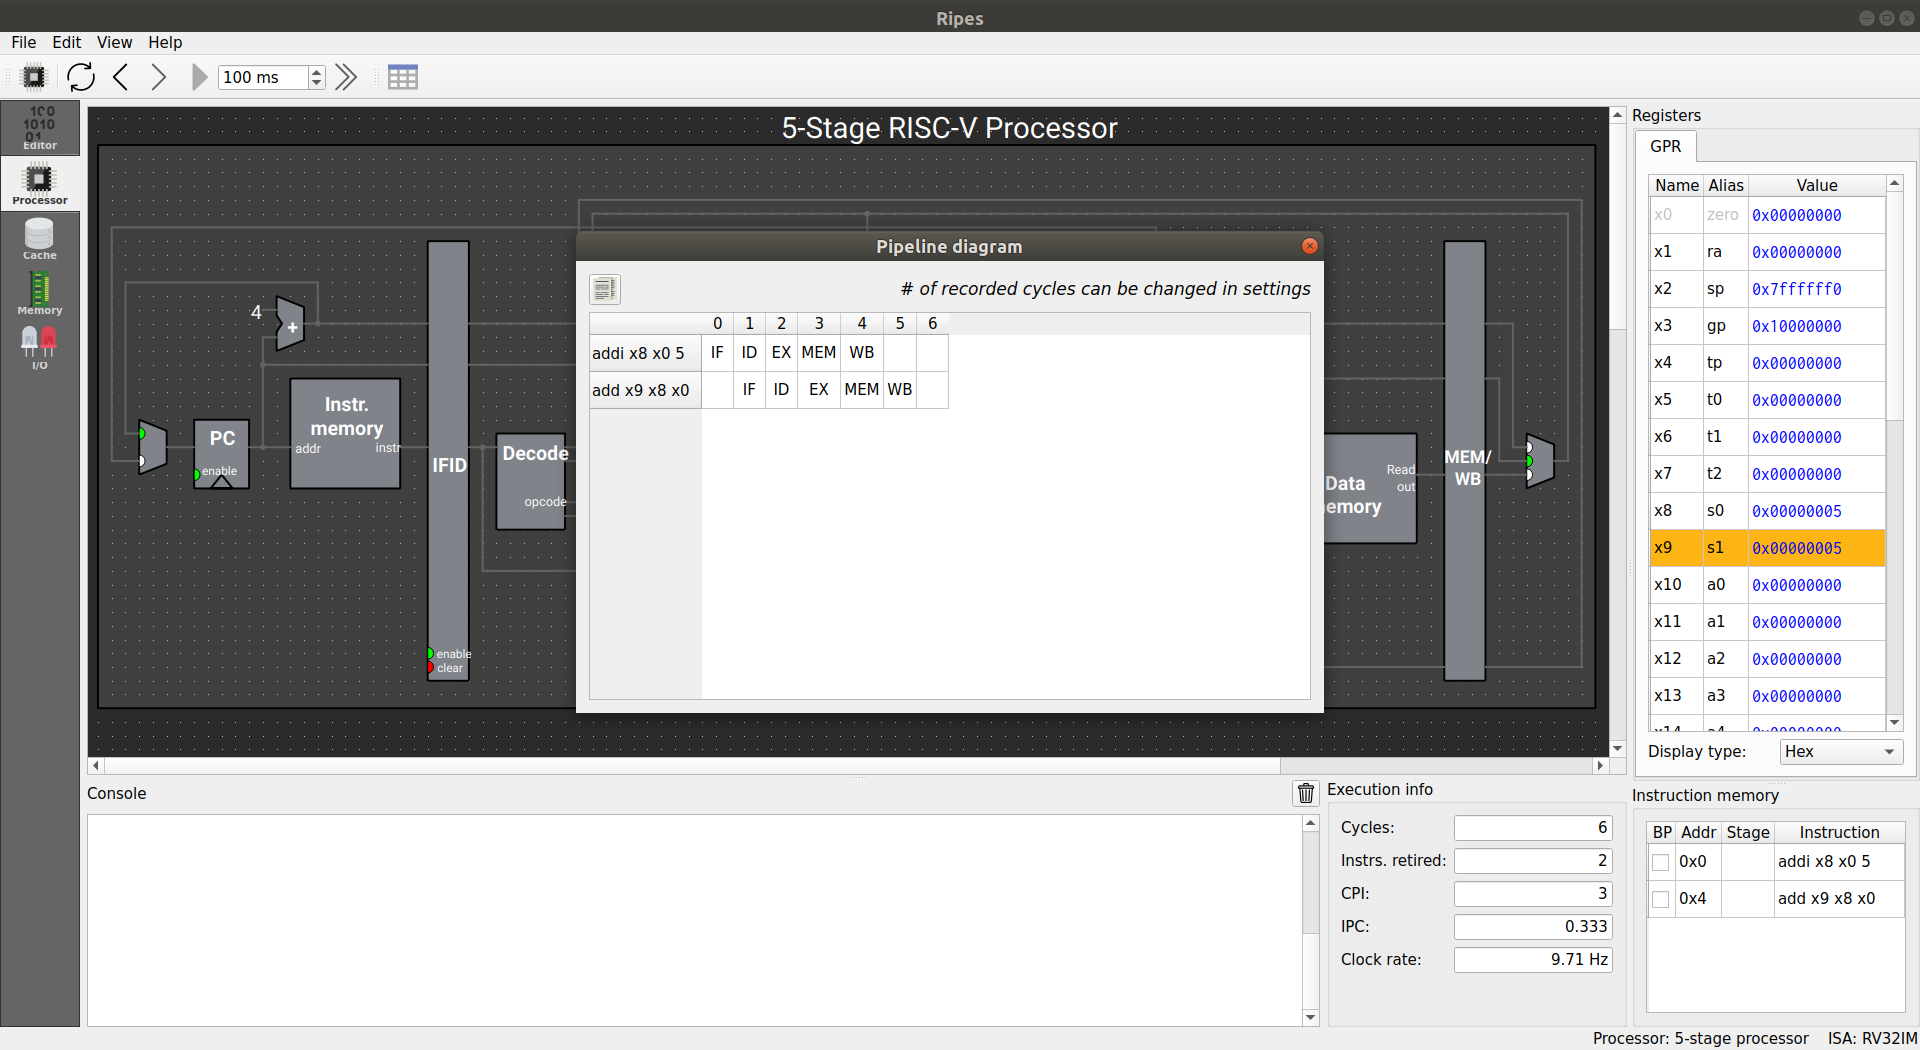
\includegraphics[scale=0.25]{Q2/a_hf_end_pipeline.png}
  \caption{With hazard detection; With forwarding;}
\end{figure}

\subsection{}
\subsubsection*{Initial Code}
\begin{verbatim}
.text

main:
    addi s0 zero 5
    add s1 s0 zero
    addi s2 zero 6
    addi s3 zero 7
\end{verbatim}

\subsubsection*{Optimized Code}
\begin{verbatim}
.text

main:
    addi s0 zero 5
    addi s2 zero 6
    addi s3 zero 7
    add s1 s0 zero
\end{verbatim}

\subsubsection*{Behaviour}
At the end of both the program, we expect registers \verb!s0! and \verb!s1! to have value 5, register \verb!s2! to have value 6 and, register \verb!s3! to have value 7.

\subsubsection*{Screenshots}
\begin{figure}[H]
  \centering
  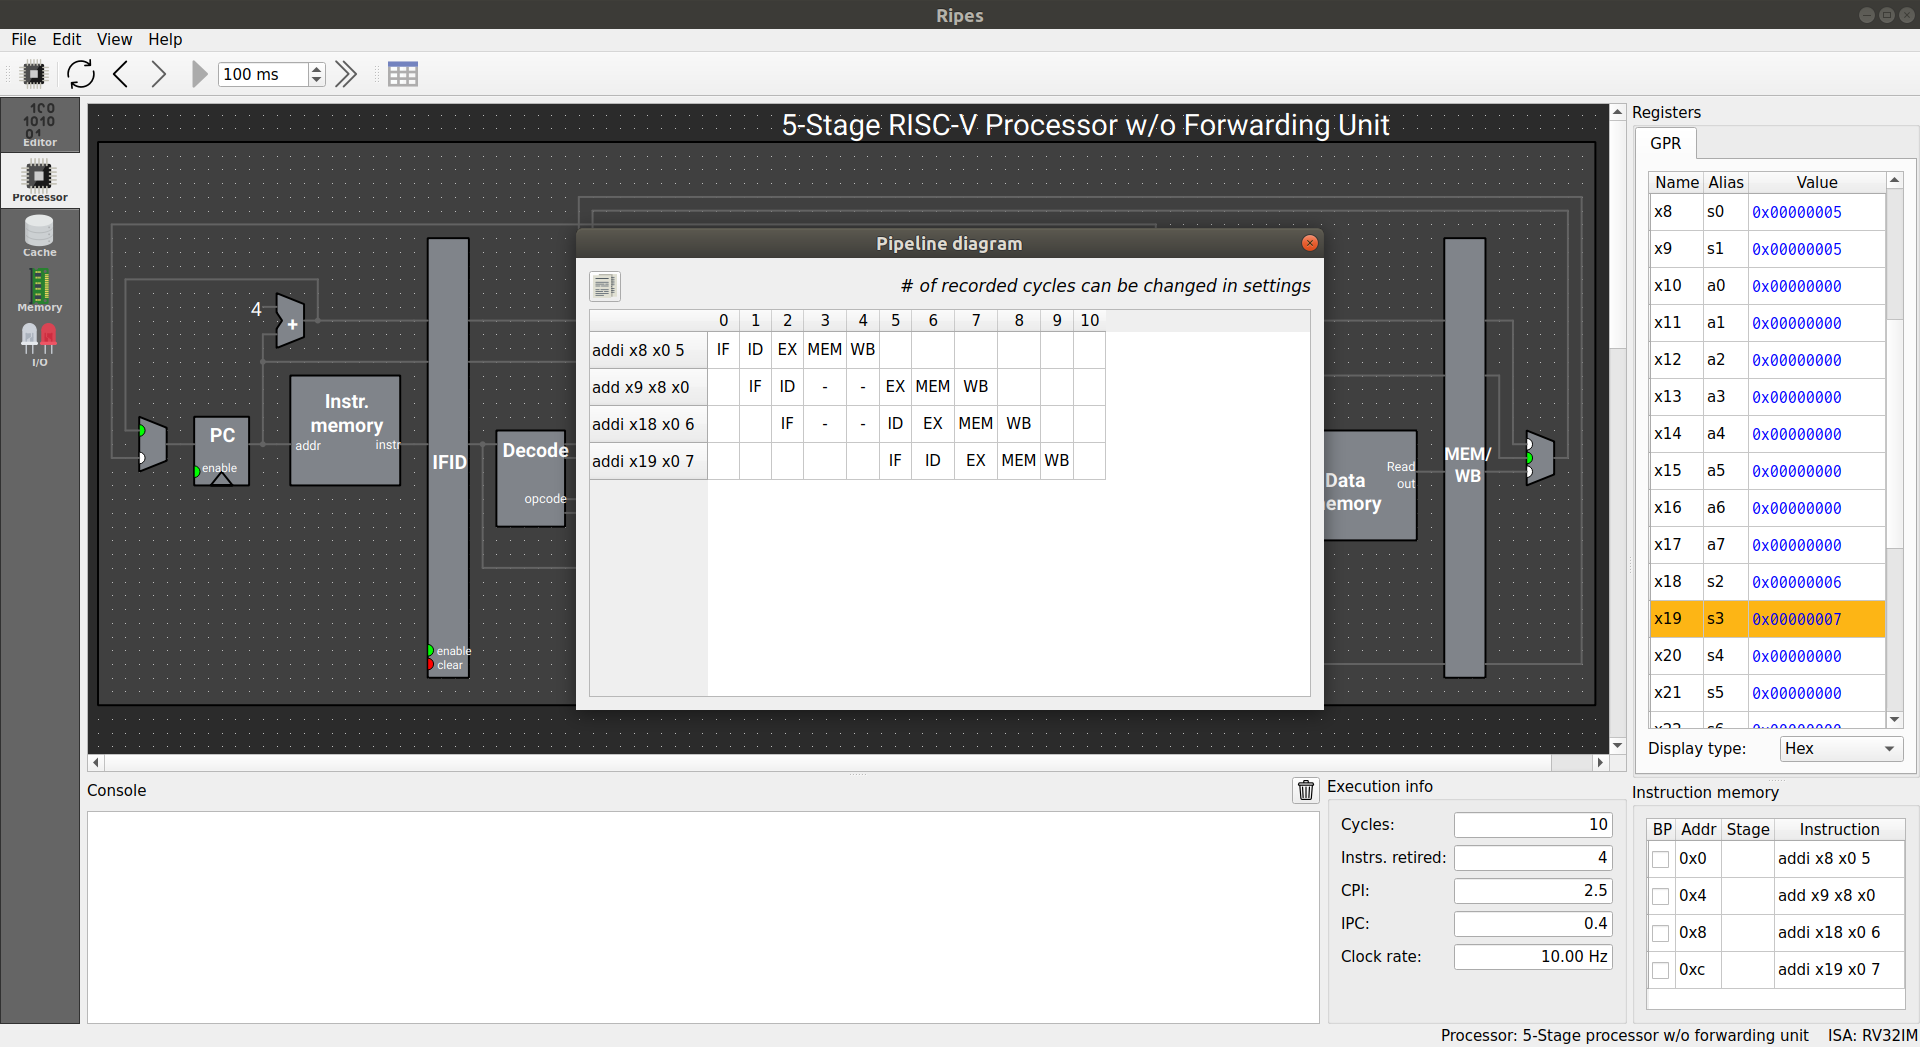
\includegraphics[scale=0.25]{Q2/b_init_hnf_end_pipeline.png}
  \caption{With hazard detection; Without forwarding; Initial code}
\end{figure}
\begin{figure}[H]
  \centering
  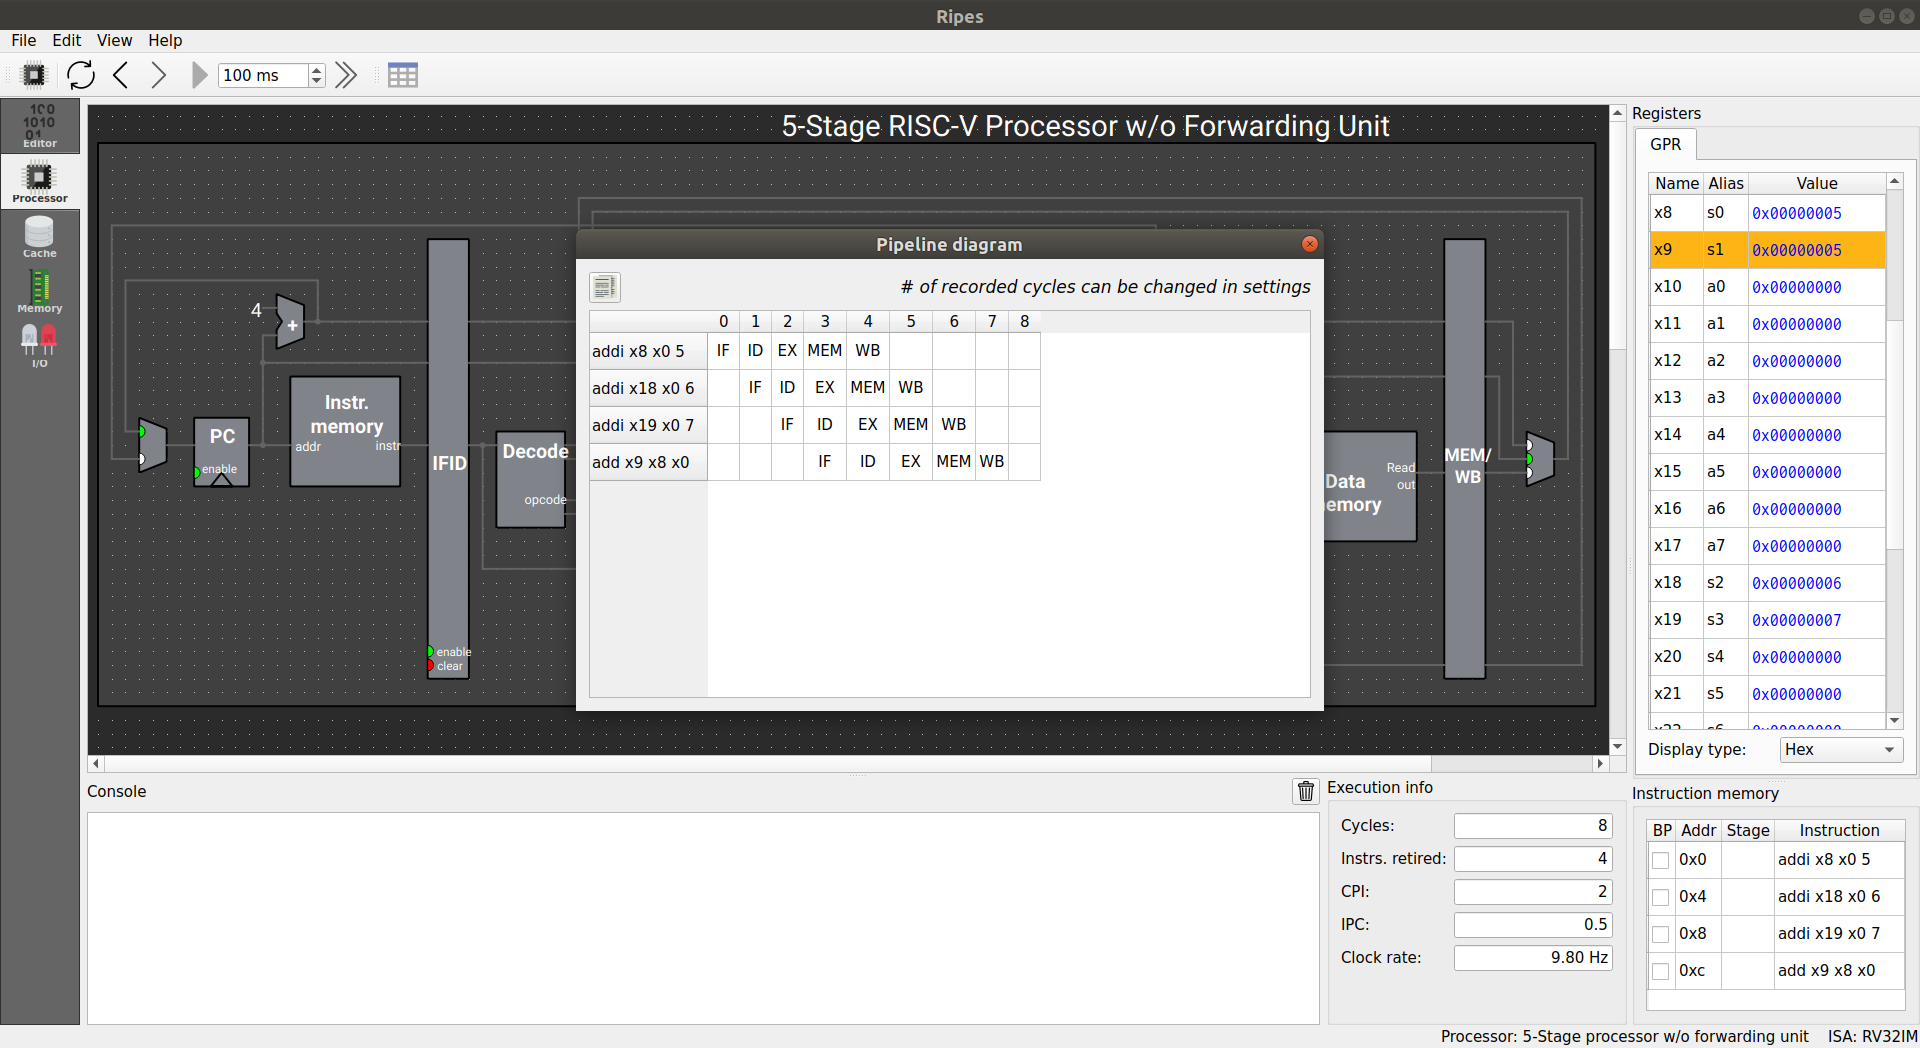
\includegraphics[scale=0.25]{Q2/b_opt_hnf_end_pipeline.png}
  \caption{With hazard detection; With forwarding; Optimized code}
\end{figure}



\end{document}
